\section{A Fine-Grained Notion of Consistency}
\label{chap:correctness:finegrained}

\mnote{Fine-grained understanding of consistency}
We have up to now given a common definition of consistency~\cite{stevens2010sosym} by enumerating consistent pairs of models in a relation.
That notion is sufficient for defining transformation networks, correctness of their artifacts, and also the essential considerations regarding orchestration, as presented in the preceding section.
Domain experts and transformation developers, however, usually think in terms of a more fine-grained notion of consistency.
They do not consider when complete models are consistent, but when specific relations between some of their elements are fulfilled, i.e., which other elements they require to exist if some elements are present in models.
For example, they consider consistency between architectural components and object-oriented classes instead of complete models containing these elements.

\mnote{Representation in transformation languages}
This is also reflected by transformation languages, such as \gls{QVTR}.
First, they require relations to be defined at the level of classes and their properties. They define how properties of some classes are related to properties of other classes.
Second, they are defined in an \emph{intensional} way, i.e., constraints specify which elements are consistent rather than enumerating all consistent instances in an \emph{extensional} specification.
We have already discussed that intensional and extensional specifications have equal expressiveness and can be transformed into each other, which is why we stick to extensional specifications for reasons of simplicity.
However, we reuse the concept of specifying relations at the level of classes and their properties.

\mnote{Benefits of fine-grained notion}
This reflects a natural understanding of consistency and, in particular, makes it easier to make statements about dependencies between consistency relations, which we need to make statements about compatibility of consistency relations.
Thus, we introduce an appropriate, fine-grained notion of consistency relations in the following.
Finally, from such a fine-grained specification, a \modellevelconsistencyrelation can always be derived by enumerating all models that fulfill all the fine-grained specifications, thus it does not restrict expressiveness in any way and can be seen as a \emph{compositional approach} for defining consistency, which is only a refinement of the notion of \modellevelconsistencyrelations.
We have presented the following definitions of a fine-grained consistency notion, partly literally, in previous work~\owncite{klare2020compatibility-report}. 
The definitions are based on those proposed in the work of \textcite[Sec. 2.3.2, 4.1.1]{kramer2017a} and \textowncite{klare2021Vitruv-JSS}.


\subsection{Fine-Grained Consistency Relations}
\label{chap:correctness:finegrained:relations}

\mnote{Conditions}
The central idea of the fine-grained consistency notion is to have consistency relations that contain pairs of objects and, broadly speaking, requires that if the objects in one side of the pair occur in a model, the others have to occur in another model as well.
A \emph{condition} encapsulates such objects, for which we require objects in another model to occur.

\begin{definition}[Condition]
    A condition $\condition{c}{}$ for a class tuple $\classtuple{C}{\condition{c}{}} = \tupled{\class{C}{\condition{c}{},1}, \dots, \class{C}{\condition{c}{},n}}$ is a set of object tuples with: 
    \begin{align*}
    &
    \forall \tupled{\object{o}{1}, \dots, \object{o}{n}} \in \condition{c}{}: \forall i \in \setted{1, \dots, n} : \object{o}{i} \in \instances{\class{C}{\condition{c}, i}}
    \end{align*}
    An element $\conditionelement{c}{} \in \condition{c}{}$ is called a \emph{condition element}.
    %
    For a model tuple $\modeltuple{m} \in \metamodeltupleinstanceset{M}$ of a metamodel tuple $\metamodeltuple{M}$ and a condition element $\conditionelement{c}{}$, we say that: 
    \begin{align*}
        &
        \modeltuple{m} \containsmath \conditionelement{c}{} \equivalentperdefinition
        \exists \model{m}{} \in \modeltuple{m} : \conditionelement{c}{} \subseteq \model{m}{}
    \end{align*}
\end{definition}

\mnote{Models containing conditions}
\emph{Conditions} represent object tuples, called \emph{condition elements}, that instantiate the same tuple of classes. 
They are supposed to occur in models that fulfill a certain condition regarding consistency and thus require elements in other models to exist, as subsequently defined by consistency relations.
We say that a tuple of models contains a condition element if any of the models contains all the objects within the condition element.
This implies that such a model's metamodel has to contain all the classes in the class tuple of the condition.
We use conditions to define consistency relations as the co-occurrence of condition elements.

\begin{definition}[Consistency Relation]
\label{def:consistencyrelation}
    Let $\classtuple{C}{l,\consistencyrelation{CR}{}}$ and $\classtuple{C}{r,\consistencyrelation{CR}{}}$ be two class tuples.
    A consistency relation $\consistencyrelation{CR}{}$ is a subset of pairs of condition elements in conditions $\condition{c}{l,\consistencyrelation{CR}{}}, \condition{c}{r,\consistencyrelation{CR}{}}$ with
    $\classtuple{C}{l,\consistencyrelation{CR}{}} = \classtuple{C}{\condition{c}{l,\consistencyrelation{CR}{}}}$ and $\classtuple{C}{r,\consistencyrelation{CR}{}} = \classtuple{C}{\condition{c}{r,\consistencyrelation{CR}{}}}$ :
    \begin{align*}
        & 
        \consistencyrelation{CR}{} \subseteq \condition{c}{l,\consistencyrelation{CR}{}} \times \condition{c}{r,\consistencyrelation{CR}{}}
    \end{align*}
    We call a pair of condition elements $\tupled{\conditionelement{c}{l}, \conditionelement{c}{r}} \in \consistencyrelation{CR}{}$ a \emph{consistency relation pair}. 
    For a model tuple $\modeltuple{m}$ and a consistency relation pair $\tupled{\conditionelement{c}{l}, \conditionelement{c}{r}}$, we say that:
    \begin{align*}
        & 
        \modeltuple{m} \containsmath \tupled{\conditionelement{c}{l}, \conditionelement{c}{r}} \equivalentperdefinition \modeltuple{m} \containsmath \conditionelement{c}{l} \land \modeltuple{m} \containsmath \conditionelement{c}{r}
    \end{align*}
\end{definition}

\mnote{Consistency relations}
A consistency relation is a set of pairs of condition elements, which indicate the tuples of objects that are considered consistent with each other. 
This means that if a model contains one of the left condition elements that occurs in the relation, another model must contain one of the related right condition elements.
It bases on two conditions that define relevant object tuples in instances of each of the two metamodels and defines the ones that are related to each other.
Without loss of generality, we assume that each condition element of both conditions occurs in at least one consistency relation pair:
\parameterizeformat{
\begin{align*}
    & 
    \forall \conditionelement{c}{} \in \condition{c}{l,\consistencyrelation{CR}{}} : \exists \tupled{\conditionelement{c}{l}, \conditionelement{c}{r}} \in \consistencyrelation{CR}{} : \conditionelement{c}{} = \conditionelement{c}{l} 
    \\ &
    \land \forall \conditionelement{c}{} \in \condition{c}{r,\consistencyrelation{CR}{}} : \exists \tupled{\conditionelement{c}{l}, \conditionelement{c}{r}} \in \consistencyrelation{CR}{} : \conditionelement{c}{} = \conditionelement{c}{r}
\end{align*}
}{}{\\ &}%

Based on these consistency relations, we can define a fine-grained notion of consistency.

\begin{definition}[Consistency] \label{def:consistency}
    Let $\consistencyrelation{CR}{}$ be a consistency relation and let $\modeltuple{m} \in \metamodeltupleinstanceset{M}$ be a tuple of models of the metamodels in $\metamodeltuple{M}$.
    We say that:
     \begin{align*}
        & 
        \modeltuple{m} \consistenttomath \consistencyrelation{CR}{} \equivalentperdefinition \\
        & \formulaskip
        \exists \consistencyrelation{W}{} \subseteq \consistencyrelation{CR}{} : 
        \bigl( \forall \tupled{\conditionelement{c}{l,1}, \conditionelement{c}{r,1}}, \tupled{\conditionelement{c}{l,2}, \conditionelement{c}{r,2}} \in \consistencyrelation{W}{} : \\
        & \formulaskip\formulaskip\formulaskip
        \tupled{\conditionelement{c}{l,1}, \conditionelement{c}{r,1}} = \tupled{\conditionelement{c}{l,2}, \conditionelement{c}{r,2}} \lor 
        ( \conditionelement{c}{l,1} \neq \conditionelement{c}{l,2} \land \conditionelement{c}{r,1} \neq \conditionelement{c}{r,2}) \bigr) \\
        & \formulaskip\formulaskip
        \land \forall \tupled{\conditionelement{c}{l}, \conditionelement{c}{r}} \in  \consistencyrelation{W}{} : \modeltuple{m} \containsmath \conditionelement{c}{l} \land \modeltuple{m} \containsmath \conditionelement{c}{r} \\
        & \formulaskip\formulaskip
        \land \forall \conditionelement{c}{l}' \in \condition{c}{l,\consistencyrelation{CR}{}} : \modeltuple{m} \containsmath \conditionelement{c}{l}' \Rightarrow \conditionelement{c}{l}' \in \condition{c}{l,\consistencyrelation{W}{}}
    \end{align*}
    We call such a $\consistencyrelation{W}{}$ a \emph{witness structure} for consistency of $\modeltuple{m}$ to $\consistencyrelation{CR}{}$, and for all pairs $\tupled{\conditionelement{w}{l}, \conditionelement{w}{r}} \in \consistencyrelation{W}{}$, we call $\conditionelement{w}{l}$ and $\conditionelement{w}{r}$ \emph{corresponding to} each other.
    
    For a set of consistency relations $\consistencyrelationset{CR} = \setted{\consistencyrelation{CR}{1}, \consistencyrelation{CR}{2}, \dots}$, we say that:
    \begin{align*}
        \formulaskip &
        \modeltuple{m} \consistenttomath \consistencyrelationset{CR} \equivalentperdefinition
        \forall \consistencyrelation{CR}{} \in \consistencyrelationset{CR} : \modeltuple{m} \consistenttomath \consistencyrelation{CR}{}
    \end{align*}
\end{definition}

\mnote{Consistency by fine-grained relations}
A consistency relation $\consistencyrelation{CR}{}$ relates one condition element at the left side to one or more other condition elements at the right side of the relation.
The definition of consistency ensures that if one condition element $\conditionelement{c}{} \in \condition{c}{l,\consistencyrelation{CR}{}}$ at the left side of the relation occurs in a tuple of models, exactly one of the condition elements related to it by a consistency relation $\consistencyrelation{CR}{}$ occurs in another model to consider the tuple of models consistent.
If another element that is related to $\conditionelement{c}{}$ occurs in the models, this one has to be, in turn, related to another condition element $\conditionelement{c}{}' \in \condition{c}{l,\consistencyrelation{CR}{}}$ of the left side of condition elements by $\consistencyrelation{CR}{}$ that also occurs in the models.
This ensures that a condition element contained in a model uniquely corresponds to another element to which it is considered consistent according to $\consistencyrelation{CR}{}$.

\begin{figure}
    \centering
    \newcommand{\hdistance}{(23em+0.5*\difftoafiveimage)}
\newcommand{\classwidth}{6em}

\begin{tikzpicture}

% Employee
\umlclassvarwidth{employee}{}{Employee\sameheight}{
name
}{\classwidth}

% Resident
\umlclassvarwidth[, right=\hdistance of employee.north, anchor=north]{resident}{}{Resident\sameheight}{
name
}{\classwidth}

% CONSISTENCY RELATIONS
\draw[directed consistency relation] (employee.east) -- node[pos=0, above right] {$e$} node[pos=0.5, below, align=center] {
$\consistencyrelation{CR}{} = \setted{ \tupled{e,r} \mid \mathvariable{e.name.toLower} = \mathvariable{r.name}}$} node[pos=1, above left] {$r$} (resident.west);

\end{tikzpicture}
    %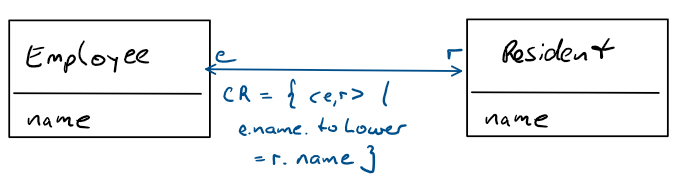
\includegraphics[width=0.8\textwidth]{figures/correctness/notion/witness_uniqueness.png}
    \caption[Example for necessity of a witness structure]{A consistency relation derived from \autoref{fig:networks:three_persons_example}, which depicts the necessity of a witness structure to ensure that only one employee out of those with differently capitalized names is allowed to correspond to a resident with the same name.}
    \label{fig:correctness:witness_uniqueness}
\end{figure}

\mnote{Witness structure}
Consider the exemplary consistency relation in \autoref{fig:correctness:witness_uniqueness}, which is derived from the one in our running example in \autoref{fig:networks:three_persons_example}.
The relation requires for each resident an employee with an appropriate name to exist and vice versa.
It assumes that resident names are stored lowercase and allows the employee name to be written in arbitrary capitalization.
Thus, for example, both the employees with names \enquote{Alice} and \enquote{alice} would be considered consistent to a resident with name \enquote{alice}.
Without the restriction defined by the auxiliary witness structure $\consistencyrelation{W}{}$, an employee model containing the employees with both capitalizations would be considered consistent to a resident model containing a corresponding resident with the same name written in lowercase.
The witness structure, however, ensures that for each employee one corresponding resident exists, thus there can only exist one employee with one of the allowed capitalizations, as each of them is corresponding to the resident with the lowercase name.
In general, the witness structure restriction ensures that if several alternatives for a corresponding element exists, only one is actually allowed to be present.

\begin{figure}
    \centering
    \newcommand{\hdistance}{20em}
\newcommand{\vdistance}{0.8em}
\newcommand{\internalvdistance}{0.3em}
\newcommand{\classwidth}{6em}
\newcommand{\objectwidth}{6.7em}
\newcommand{\leftshift}{5em}

\begin{tikzpicture}[
    witness/.style={consistency relation, latex-latex},
    witness fault/.style={witness, color=darkred, dashed}
]

% Employee
\umlclassvarwidth{employee}{}{Employee\sameheight}{
name
}{\classwidth}

% Resident
\umlclassvarwidth[, right=\hdistance of employee.north, anchor=north]{resident}{}{Resident\sameheight}{
name
}{\classwidth}

% CONSISTENCY RELATIONS
\draw[directed consistency relation] (employee.east) -- node[pos=0, above right] {$e$} node[pos=0.5, below, align=center] {
$\begin{aligned}
    \consistencyrelation{CR}{} = \setted{ \tupled{e,r} \mid \mathvariable{e.name} = \mathvariable{r.name} \\[-0.4em]
	\lor \mathvariable{e.name.toLower} = \mathvariable{r.name} }
\end{aligned}$} node[pos=1, above left] {$r$} (resident.west);

% EXAMPLE 1
% Employee
\umlobjectvarwidth[, below right=2.2*\vdistance and \leftshift of employee.south west, anchor=north west]{instance1_employee}{}{Employee\sameheight}{
	name = "Alice"
}{\objectwidth}
% Resident
\umlobjectvarwidth[, below=2.2*\vdistance of resident.south east, anchor=north east]{instance1_resident}{}{Resident\sameheight}{
	name = "Alice"
}{\objectwidth}

% EXAMPLE 2
% Employee
\umlobjectvarwidth[, below=\vdistance of instance1_employee.south, anchor=north]{instance2_employee}{}{Employee\sameheight}{
	name = "Alice"
}{\objectwidth}
% Resident
\umlobjectvarwidth[, below=\vdistance of instance1_resident.south, anchor=north]{instance2_resident}{}{Resident\sameheight}{
	name = "alice"
}{\objectwidth}


% EXAMPLE 3
% Employee
\umlobjectvarwidth[, below=\vdistance of instance2_employee.south, anchor=north]{instance3_employee1}{}{Employee\sameheight}{
	name = "alice"
}{\objectwidth}
\umlobjectvarwidth[, below=\internalvdistance of instance3_employee1.south, anchor=north]{instance3_employee2}{}{Employee\sameheight}{
	name = "Alice"
}{\objectwidth}
% Resident
\umlobjectvarwidth[, below=\vdistance of instance2_resident.south, anchor=north]{instance3_resident1}{}{Resident\sameheight}{
	name = "alice"
}{\objectwidth}
\umlobjectvarwidth[, below=\internalvdistance of instance3_resident1.south, anchor=north]{instance3_resident2}{}{Resident\sameheight}{
	name = "Alice"
}{\objectwidth}

% EXAMPLE 4
% Employee
\umlobjectvarwidth[, below=\vdistance of instance3_employee2.south, anchor=north]{instance4_employee1}{}{Employee\sameheight}{
	name = "Alice"
}{\objectwidth}
% Resident
\umlobjectvarwidth[, below=\vdistance of instance3_resident2.south, anchor=north]{instance4_resident1}{}{Resident\sameheight}{
	name = "Alice"
}{\objectwidth}
\umlobjectvarwidth[, below=\internalvdistance of instance4_resident1.south, anchor=north]{instance4_resident2}{}{Resident\sameheight}{
	name = "John"
}{\objectwidth}

% EXAMPLE 5
% Resident
\umlobjectvarwidth[, below=\vdistance of instance4_resident2.south, anchor=north]{instance5_resident1}{}{Resident\sameheight}{
	name = "Alice"
}{\objectwidth}
\umlobjectvarwidth[, below=\internalvdistance of instance5_resident1.south, anchor=north]{instance5_resident2}{}{Resident\sameheight}{
	name = "alice"
}{\objectwidth}
% Employee
\umlobjectvarwidth[, left=\hdistance-\leftshift+(\classwidth-\objectwidth) of instance5_resident1.north, anchor=north]{instance5_employee1}{}{Employee\sameheight}{
	name = "Alice"
}{\objectwidth}

% EXAMPLE 6
% Resident
\umlobjectvarwidth[, below=\vdistance of instance5_resident2.south, anchor=north]{instance6_resident1}{}{Resident\sameheight}{
	name = "alice"
}{\objectwidth}
% Employee
\umlobjectvarwidth[, left=\hdistance-\leftshift+(\classwidth-\objectwidth) of instance6_resident1.north, anchor=north]{instance6_employee1}{}{Employee\sameheight}{
	name = "alice"
}{\objectwidth}
\umlobjectvarwidth[, below=\internalvdistance of instance6_employee1.south, anchor=north]{instance6_employee2}{}{Employee\sameheight}{
	name = "Alice"
}{\objectwidth}

\node[left=0.5*\leftshift of instance1_employee.west] {\textbf{1.}};
\node[left=0.5*\leftshift of instance2_employee.west] {\textbf{2.}};
\node[left=0.5*\leftshift of instance3_employee1.west] {\textbf{3.}};
\node[left=0.5*\leftshift of instance4_employee1.west] {\textbf{4.}};
\node[left=0.5*\leftshift of instance5_employee1.west] {\textbf{5.}};
\node[left=0.5*\leftshift of instance6_employee1.west] {\textbf{6.}};

\draw ([xshift=-\leftshift,yshift=0.5*\vdistance]instance1_employee.north west) -- ([yshift=0.5*\vdistance]instance1_resident.north east); 
\draw ([xshift=-\leftshift,yshift=0.5*\vdistance]instance2_employee.north west) -- ([yshift=0.5*\vdistance]instance2_resident.north east); 	 
\draw ([xshift=-\leftshift,yshift=0.5*\vdistance]instance3_employee1.north west) -- ([yshift=0.5*\vdistance]instance3_resident1.north east); 	 
\draw ([xshift=-\leftshift,yshift=0.5*\vdistance]instance4_employee1.north west) -- ([yshift=0.5*\vdistance]instance4_resident1.north east); 	 
\draw ([xshift=-\leftshift,yshift=0.5*\vdistance]instance5_employee1.north west) -- ([yshift=0.5*\vdistance]instance5_resident1.north east); 
\draw ([xshift=-\leftshift,yshift=0.5*\vdistance]instance6_employee1.north west) -- ([yshift=0.5*\vdistance]instance6_resident1.north east); 	


% WITNESS STRUCTURE
\draw[witness] (instance1_employee) -- (instance1_resident);
\draw[witness] (instance2_employee) -- (instance2_resident);
\draw[witness] (instance3_employee1) -- (instance3_resident1);
\draw[witness] (instance3_employee2) -- (instance3_resident2);
\draw[witness] (instance4_employee1) -- (instance4_resident1);
\draw[witness fault] (instance5_employee1) -- (instance5_resident1);
\draw[witness fault] (instance5_employee1) -- (instance5_resident2);
\draw[witness fault] (instance6_employee1) -- (instance6_resident1);
\draw[witness fault] (instance6_employee2) -- (instance6_resident1);

\end{tikzpicture}
    \caption[Examples for fine-grained consistency relations]{A consistency relation between employee and resident and six example model pairs: pairs 1--4 consistent with an appropriate witness structure $\consistencyrelation{W}{}$ shown in blue, solid lines, and pairs 5 and 6 inconsistent with an inappropriate mapping structure shown in red, dashed lines. Adapted from~\owncite[Fig.~2]{klare2020compatibility-report}.}
    \label{fig:correctness:consistency_example}
\end{figure}

\begin{example}
The definition of consistency is exemplified in \autoref{fig:correctness:consistency_example}, which is an alternation of an extract of \autoref{fig:networks:three_persons_example} only considering employees and residents. Models with employees and residents are considered consistent if for each employee exactly one resident with the same name or the name in lowercase exists.
The model pairs $1$--$3$ are obviously consistent according to the definition, because there is always a pair of objects that fulfills the consistency relation.
In model pair $4$, there is a consistent resident for each employee, but there is no appropriate employee for the resident with $\mathvariable{name} = "\mathvariable{Bob}"$. However, our definition of consistency only requires that for each condition element at the left side of the relation that appears in the models, an appropriate right element occurs, but not vice versa. Thus, a relation is interpreted unidirectionally, which we subsequently discuss in more detail.
In model pair $5$, there are two residents with names in different capitalizations, which would both be considered consistent to the employee according to the consistency relation.
Comparably, in model pair $6$, there is a resident that fulfills the consistency relations for both employees, each having a different but matching capitalization. 
However, the consistency definition requires that each model element for which consistency is defined by a consistency relation must only have one corresponding element. 
In this case, there are two residents or employees that could be considered consistent to the employee or resident, respectively, thus there is no witness structure with a unique mapping between the elements as required by the definition.
\end{example}

\mnote{Unidirectional notion}
As mentioned in the example, the definition considers consistency in a unidirectional way, which means that a consistency relation may define that some elements $\conditionelement{c}{r}$ are required to occur in a tuple of models if some elements $\conditionelement{c}{l}$ occur, but not vice versa.
Such a unidirectional notion can also be reasonable in our example, as it could make sense to require a resident for each employee, but not every resident might be employed and thus also represent an employee.
To achieve a bijective consistency definition, for each consistency relation $\consistencyrelation{CR}{}$ its transposed relation $\consistencyrelation{CR}{}^T = \setted{\tupled{\conditionelement{c}{l}, \conditionelement{c}{r}} \mid \tupled{\conditionelement{c}{r}, \conditionelement{c}{l}} \in \consistencyrelation{CR}{}}$ can be considered as well.
Regarding \autoref{fig:correctness:consistency_example}, if we consider the relation between employees and residents as well as its transposed, the model pair $4$ would also be considered inconsistent, because an appropriate employee for each resident is required by the transposed relation.
We call sets of consistency relations that contain only bijective definitions of consistency \emph{symmetric}.

\begin{definition}[Symmetric Consistency Relation Set]
    Let $\consistencyrelationset{CR}$ be a set of consistency relations.
    We say that $\consistencyrelationset{CR}$ is \emph{symmetric} if, and only if, for each contained relation its transposed one is also contained:
    \begin{align*}
        &
        \consistencyrelationset{CR} \mathtextspacearound{is symmetric} \equivalentperdefinition
        \forall \consistencyrelation{CR}{} \in \consistencyrelationset{CR} :
        \consistencyrelation{CR}{}^T \in \consistencyrelationset{CR}
    \end{align*}
\end{definition}

\mnote{Reasons for unidirectionality}
Any description of bijective consistency relations can be defined with a symmetric consistency relation set.
We have defined consistency in a unidirectional way for the two following reasons.
\begin{longenumerate}
    \item Some relevant consistency relations are actually not bijective. 
    Apart from the simple example concerning residents and employees, this situation always occurs when objects at different levels of abstraction are related.
    Consider a relation between components and classes, requiring for each component an implementation class but not vice versa, or a relation between \gls{UML} models and object-oriented code, requiring for each \gls{UML} class an appropriate class in code but not vice versa.
    These relations could not be expressed if consistency relations were always considered bijective.
    \item We consider networks of consistency relations, in which a combination of multiple bijective consistency relations does not necessarily imply a bijective consistency relation again. 
    Thus, we need a unidirectional notion of consistency relations anyway.
\end{longenumerate}

\mnote{Explicit trace models}
One might argue that consistency is usually traced by means of a \emph{trace model}, which stores the pairs of element tuples in models that fulfill a consistency relation.
A trace model can be seen as an explicit representation of a witness structure as specified in \autoref{def:consistency}.
We do, however, not explicitly consider such an explicit trace model in this formalism for two reasons also discussed in previous work~\owncite{klare2021Vitruv-JSS}.
First, a trace model is only necessary in practice if no identifying information for related elements is present, or if performance is to be improved.
However, we assume such identifying information to exist without loss of generality, as introduced in \autoref{chap:networks:models:assumption}.
Second, a trace model can, from a theoretical perspective, be treated as a usual model by defining consistency between one concrete and one trace model. This conforms to the fact that each multiary relation can be expressed by binary relations to an additional model (in this case the trace model), as discussed in existing work~\cite{stevens2020BidirectionalTransformationLarge-SoSym, cleve2019dagstuhl}.
We discuss practical benefits of having an explicit trace model for consistency preservation in \autoref{chap:synchronization} to distinguish modifications of elements from their removal and addition.
But this does, as discussed, not restrict applicability of our formalism.


\subsection{Expressiveness of Fine-Grained Relations} % Equivalence to \modellevelconsistencyrelations

\mnote{Expressiveness of fine-grained consistency}
The model-level consistency notion of \autoref{def:modellevelconsistency} is established and based on notions used by several researchers.
The fine-grained consistency notion according to \autoref{def:consistency} is based on the insight that practical approaches to describe consistency and its preservation use fine-grained rules rather than enumerating consistent model pairs.
We did, however, only provide examples that justify specific decisions in the definitions, such as the witness structure for corresponding elements, but we did not argue if and why fine-grained relations are an actual refinement, such that statements about \modellevelconsistencyrelations also apply to fine-grained relations.

\mnote{Implication of model-level relation}
To show that every set of fine-grained consistency relations can be expressed by a single \modellevelconsistencyrelation, we can use the same constructive approach that we have used to define consistency according to multiple consistency relations, be they at the model level or fine-grained.
Given fine-grained consistency relations $\consistencyrelationset{CR} = \setted{\consistencyrelation{CR}{1}, \dots, \consistencyrelation{CR}{k}}$, we can construct an equivalent \modellevelconsistencyrelation $\consistencyrelation{CR}{}$ as follows:
\begin{align*}
    \consistencyrelation{CR}{} = \setted{\modeltuple{m} \mid \modeltuple{m} \consistenttomath \consistencyrelationset{CR}}
\end{align*}

\mnote{Model-level relations more expressive}
A \modellevelconsistencyrelation can, however, not necessarily be expressed by fine-grained consistency relations.
The most simple construction approach would define a single fine-grained consistency relation to express a \modellevelconsistencyrelation, which contains the complete models instead of extracts of them.
The definition of consistency is, however, different for the two types of relations.
While at the model level consistency is defined as two (or more) models being in a relation (see \autoref{def:modellevelconsistency}), fine-grained consistency relations do only describe that if an element at the left side of the relation occurs in a model, then any of the related elements at the right side has to occur in another.
If two models are considered consistent by a \modellevelconsistencyrelation, they are also consistent to the accordingly constructed fine-grained relation, because there is a witness structure that contains exactly the two consistent models.
If there is a model that is not considered consistent to any other model in the \modellevelconsistencyrelation, thus the \modellevelconsistencyrelation does not contain any pair with that model, then there will also be no such pair in the fine-grained relation.
According to \autoref{def:consistency} of consistency for fine-grained relations, if there is no condition element in the relation, then consistency is not constrained for the contained model elements.
In consequence, such a model would be considered consistent to every other model.

\mnote{Additional semantics in consistency relations}
While, at first, this may seem inappropriate, it actually is appropriate for two reasons.
First, the formalism can only express that for some elements other elements need to exist, but not that specific elements are not allowed to exist if other elements exist.
This is reasonable, because consistency between models is supposed to ensure that the overlap of information is represented uniformly, thus to express that information in one model needs to be represented in another one as well.
Expressing that some elements are not allowed to exist because of others, e.g., being an employee in one model, the same person cannot be a student in another model, is actually not a consistency constraint for information shared between models.
This is actually additional information that should be stored in a specific model representing these semantics.
Thus, we do not consider this case at all.

\mnote{Restriction of valid models}
Second, the formalism for fine-grained consistency relations can not prevent specific elements from existing at all.
For example, a consistency relation may define that for a component in an architecture model a corresponding class in the object-oriented design model has to exist, but it may not restrict that only components of specific names are allowed.
Such restrictions should and actually are separate specifications not related to consistency between models but restricting a model on its own.
Thus, the metamodel or some additional specification for it should provide such restrictions of valid models, which we have discussed as a restriction of $\metamodelinstanceset{M}{}$ for a metamodel $\metamodel{M}{}$ in \autoref{chap:networks:models}.

\mnote{Insight transferability between notions}
Summarizing, we found that we can express each set of fine-grained consistency relations by a \modellevelconsistencyrelation.
Additionally, we know that there are specific kinds of restrictions that can be encoded in \modellevelconsistencyrelations but not in fine-grained consistency relations.
We have, however, discussed why they are not relevant for the designated application area of consistency preservation.
In consequence, all insights made for \modellevelconsistencyrelations can also be applied to fine-grained consistency relations and, if specific restrictions are excluded, vice versa.

%\begin{itemize}
    %\item Is compatibility a subclass of correctness? Is every correct set of relations compatible as well?
    %\item Problematisch: unser Konsistenzbegriff für Relationen (feingranulare Relationen) schließt keine Modelle aus, der Konsistenzbegriff hier aber schon. Wie realisiere ich die feingranularen Relationen, die dafür sorgen, dass nur genau ein Tupel von Modellen konsistent ist?
    %\item Wir müssen bei der Ableitung unseres Kompatibilitätsbegriffes erklären, dass bei uns der vollständige Ausschluss bestimmter Modelle nicht Teil einer feingranularen Konsistenzrelation sein darf, sondern Teil einer weiteren Spezifikation, die angibt, welche Modelle überhaupt valide sind. Denn so ist es in Transformationssprachen tatsächlich auch.
%\end{itemize}


\subsection{Application to Consistency Preservation Rules}
\label{chap:correctness:finegrained:rules}

\mnote{Fine-grained notion in transformation languages}
As mentioned before, the fine-grained notion of consistency fits well to how transformation languages consider consistency.
They allow to define rules that relate only some classes by relations, conforming to fine-grained consistency relations, from which fine-grained consistency preservation rules are derived.
Alternatively, they directly allow to define rules to preserve consistency between specific classes.
These rules are often called \emph{transformation rules} and composed to a transformation that consists of multiple such rules, each encoding a consistency relation and a preservation rule.

\mnote{Conflicts between transformation rules}
It may easily happen that the execution of one transformation rule leads to the violation of the consistency relation of another, which induces dependencies between the individual transformation rules.
Thus, a combination of transformation rules to a transformation has to ensure correctness, i.e., that the consecutive execution of the rules leads to a consistent state of the models.
Languages such as \gls{QVTR} and \gls{QVTO} therefore specify that transformation rules may not be conflicting~\cite[7.10.2.]{qvt}.
It is also a dedicated topic of research to ensure that the rules of a single transformation conform to each other, e.g.~\cite{cuadrado2017tse,cabot2010VerificationInvariants-JSS}, which is why we assume that transformations fulfill that property.

\mnote{Extension of Consistency preservation rules}
To avoid the necessity of specifying this conformance property for transformation rules, we stick to the existing notion of coarse-grained consistency preservation rules, as it is sufficient for our considerations.
Still, consistency preservation rules were defined for \modellevelconsistencyrelations in \autoref{def:consistencypreservationrule}.
This can, however, be easily extended to fine-grained consistency relations, as we simply need to require the rule to consider consistency to a set of fine-grained relations according to \autoref{def:consistency} rather than consistency to a single \modellevelconsistencyrelation according to \autoref{def:modellevelconsistency}.

\begin{figure}
    \centering
    \newcommand{\hdistance}{17em}
\newcommand{\vdistance}{6.2em}

\begin{tikzpicture}[
    model style/.style={color=darkgray},
    concept/.style={draw, minimum width=8.5em, minimum height=3em, inner sep=0.5em},
    model concept/.style={model style, concept},
    metamodel concept/.style={concept, align=center},
    model relation/.style={model style},
    metamodel relation/.style={},
]

%\node[model concept, minimum height=1.5em, minimum width=6em] (model) {Model};
%\node[metamodel concept, minimum height=1.5em, minimum width=6em, right=0.7*\hdistance of model.north, anchor=north] (metamodel) {Metamodel};

\node[metamodel concept, minimum height=1.5em] (metamodel) {Metamodel};

\node[metamodel concept, below left=0.9*\vdistance and 0.5*\hdistance of metamodel.north, anchor=north] (mlcr) {Model-Level\\ Consistency Relation};
\node[metamodel concept, below right=0.9*\vdistance and 0.5*\hdistance of metamodel.north, anchor=north] (cr) {(Fine-Grained)\\ Consistency Relation};
\node[metamodel concept, below=1.15*\vdistance of mlcr.north, anchor=north] (cpr) {Consistency\\ Preservation Rule};
\node[metamodel concept, below=1.15*\vdistance of cr.north, anchor=north] (transformation) {Transformation};
\node[metamodel concept, below=\vdistance of transformation.north, anchor=north] (orchestration) {Orchestration\\ Function};
\node[metamodel concept, below=\vdistance of orchestration.north, anchor=north] (network) {Transformation\\ Network};
\node[metamodel concept, left=\hdistance of orchestration.north, anchor=north] (application) {Application\\ Function};

%\draw[model relation, dashed, -angle 60] (model) -- node[uml cardinality start, pos=0, below right] {*} node[uml association name, above] {\guillemotleft instance of\guillemotright} node[uml cardinality end, pos=1, below left] {1} (metamodel);

\draw[metamodel relation, open diamond-angle 60] (mlcr) -- node[uml cardinality start, pos=0, above right=0em and 1em] {*} node[uml association name, pos=0.35, above left=0em and -0.3em, align=center] {describes\\ consistency\\ between} node[uml cardinality end, pos=1, below right] {2} ([xshift=-1.5em]metamodel.south);
\draw[metamodel relation, open diamond-angle 60] (cr) -- node[uml cardinality start, pos=0, above left=0em and 1em] {*} node[uml association name, pos=0.35, above right=0em and -0.3em, align=center] {describes\\ consistency\\ between} node[uml cardinality end, pos=1, below left] {2} ([xshift=1.5em]metamodel.south);
\draw[metamodel relation, -angle 60] (cr) -- node[uml cardinality start, pos=0, below left] {*} node[uml association name, above, align=center] {implies} node[uml cardinality end, pos=1, below right] {1} (mlcr);

\coordinate (crosspoint) at ($(cpr)!0.5!(cr)$);
\draw[metamodel relation, -angle 60] (crosspoint) -- node[uml role start, pos=0, above=0.5em] {either or} node[uml cardinality end, pos=1, below left] {1} (mlcr);
\draw[metamodel relation, -angle 60] (crosspoint) -- node[uml cardinality end, pos=1, below right] {1..*} (cr);
\draw[metamodel relation, dashed] ([xshift=-2em]crosspoint) -- ([xshift=2em]crosspoint);
\draw[metamodel relation, -angle 60] ([yshift=0.3em]cpr.east) -| node[uml cardinality start, pos=0, above right=0em] {*} node[uml association name, pos=1, below left, align=center] {preserves\\ consistency\\ to} ([xshift=-0.5em]crosspoint);
\draw[metamodel relation, -angle 60] ([yshift=0.3em]transformation.west) -| node[uml cardinality start, pos=0, above left] {*} node[uml association name, pos=1, below right, align=center] {consists\\ of} ([xshift=0.5em]crosspoint);
\draw[metamodel relation, open diamond-angle 60] ([yshift=-0.5em]transformation.west) -- node[uml cardinality start, pos=0, below left] {*} node[uml association name, pos=0.5, below, align=center] {consists of} node[uml cardinality end, pos=1, below right] {1} ([yshift=-0.5em]cpr.east);

\draw[metamodel relation, -angle 60] (orchestration) -- node[uml cardinality start, pos=0, above left] {*} node[uml association name, right] {orchestrates} node[uml cardinality end, pos=1, below left] {*} (transformation);
\draw[metamodel relation, -angle 60] (application) -- node[uml cardinality start, pos=0, above left] {*} node[uml association name, above, pos=0.35, sloped] (executes_label) {executes} node[uml cardinality end, pos=1, below right] {*} (transformation);
\draw[metamodel relation, densely dashed] (executes_label) -- node[uml association name, below, sloped] {orchestrated by} node[uml cardinality end, pos=1, above left=0.5em and 0em] {1} (orchestration.west);

\draw[metamodel relation, open diamond-angle 60] (network) -- node[uml cardinality start, pos=0, above left] {*} node[uml association name, right] {consists of} node[uml cardinality end, pos=1, below left] {1} (orchestration);
\draw[metamodel relation, open diamond-angle 60] (network.west) -- node[uml cardinality start, pos=0, above left] {*} node[uml association name, above, sloped] {consists of} node[uml cardinality end, pos=1, below left] {1} (application);
\draw[metamodel relation, open diamond-angle 60] (network.east) -- node[uml cardinality start, pos=0, above right] {*} ++(2em, 0) |- node[uml association name, pos=0.25, sloped, above, align=center] {consists of} node[uml cardinality end, pos=1, above right] {*} (transformation.east);


\end{tikzpicture}

    %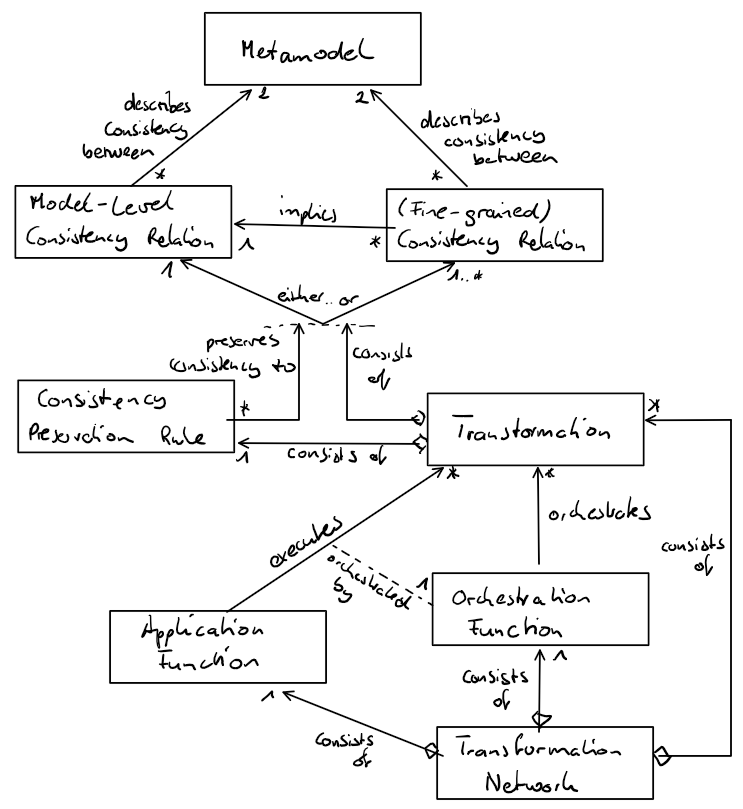
\includegraphics[width=0.85\textwidth]{figures/correctness/notion/conceptual_model.png}
    \caption[Conceptual model for transformation networks]{A conceptual model for the terms and artifacts introduced for transformation networks and their relations. Adapted from~\owncite[Fig.~5]{klare2021Vitruv-JSS}.}
    \label{fig:correctness:conceptual_model}
\end{figure}

\mnote{Consistency preservation for fine-grained relations}
A consistency preservation rule $\consistencypreservationrule{\consistencyrelationset{CR}}$ for a set of consistency relations $\consistencyrelationset{CR}$ according to \autoref{def:consistencyrelation} is thus still considered correct if it only returns changes when they yield models that are consistent to all consistency relations if applied to the input models, in accordance with \autoref{def:consistencypreservationrulecorrectness}:
\begin{align*}
    &
    \forall \model{m}{1} \in \metamodelinstanceset{M}{1}, \model{m}{2} \in \metamodelinstanceset{M}{2}, \change{\metamodel{M}{1}} \in \changeuniverse{\metamodel{M}{1}}, \change{\metamodel{M}{2}} \in \changeuniverse{\metamodel{M}{2}} : \\
    & \formulaskip
    \big( \exists \change{\metamodel{M}{1}}' \in \changeuniverse{\metamodel{M}{1}}, \change{\metamodel{M}{2}}' \in \changeuniverse{\metamodel{M}{2}} : \tupled{\change{\metamodel{M}{1}}', \change{\metamodel{M}{2}}'} = \consistencypreservationrule{\consistencyrelationset{CR}}(\model{m}{1}, \model{m}{2}, \change{\metamodel{M}{1}}, \change{\metamodel{M}{2}}) \\
    & \formulaskip\formulaskip
    \Rightarrow \tupled{\change{\metamodel{M}{1}}'(\model{m}{1}),\change{\metamodel{M}{2}}'(\model{m}{2})} \consistenttomath \consistencyrelationset{CR} \big)
\end{align*}
Note that being consistent to all fine-grained consistency relations is equivalent to being consistent to the \modellevelconsistencyrelation induced by the fine-grained relations.

\mnote{Transformations for fine-grained relations}
Likewise, we consider a synchronizing transformation according to \autoref{def:synchronizingtransformation} as a pair of fine-grained consistency relations and a consistency preservation rule for them, thus $\transformation{t} = \tupled{\consistencyrelationset{CR}, \consistencypreservationrule{\consistencyrelationset{CR}}}$.
Again, in conformance with \autoref{def:synchronizingtransformationcorrectness}, we call such a transformation $\transformation{t}$ correct if, and only if, its consistency preservation rule is correct.
